%!TEX root = ../../report.tex
\chapter{Construction process} % (fold)
\label{cha:implementation}
This chapter is dedicated to explain the process of manufacturing and assembling the introduced designs.
From the important role of emerging low-cost technologies like FFF 3D printing up to the creation of custom PCBs for reducing the weight of the robot, the following sections are meant to explain the process of acquisition and construction of all the components of RuBi presented in previous chapters.
The implementation of the final prototype has always been led by criteria of security, constrained budget and feasibility for maintenance and futures improvements.

%!TEX root = ../../../report.tex
\section{3D printing} % (fold)
\label{sec:3d_printing}
The parts modeled for the project and shown in section \ref{sub:computer_aided_design}, contain complex geometries that can only be achieved by 3D printing or complex machining.
Due to its availability and low price, Fused Filament Fabrication (FFF) technology has been used to implement the parts although other methods were considered.
The goals of this project requires the use of rapid and low-cost prototyping. 
Due to its intrinsic iterative design and the constrained timing, a technology that allows fast modifications in the design is required.

The additive manufacturing (AM) refers to the process of creating a geometry by adding material.
Besides FFF, others technologies as Stereolithography (SLA) or Digital Light Processing (DLP) that make use of the light to solidify a photo-sensible liquid, generally give better accuracy but at the expense of a higher price.
In this line, powder based AM like Selective laser melting (SLM) and Selective laser sintering (SLS), give also a higher detail although the post-processing and posterior mechanical properties tend to be lower.

Inside of the FFF, there are several materials from which a part can be printed of.
Stand out polymers like Polylactide (PLA) and Acrylonitrile butadiene styrene (ABS), materials easily printable that have good physical properties.
Its price can be considered inexpensive when comparing with the other AM technologies presented.
The easy access to this technology, mainly powered by its low-cost tag, has caused an increase of the popularity of this kind of 3D printing giving as a result a big community.
The outcome of this has been a wide variety of printable filaments with exotic properties: from non-flamable PLA to carbon fiber reinforced parts with metal-like mechanical properties.

For this project FFF using PLA has been used.
The reasons are feasibility and rapidness.
The availability of multiple 3D printers and filaments made the selection of this technology straightforward.
The 3D printer used is a M Prime One \cite{m_prime_one} with a 0.4 mm noozle.
PLA of two different colors was available, Blue and Black (the color may change the mechanical properties of the final printed part, due to different additives are used), from the provider BQ.
All the parts have been printed at 0.2 mm layer height making use of free software slicers as Cura \cite{cura} and Slic3r \cite{slic3r}.
The Figure \ref{fig:3d_printing_gcode} shows the gcode visualization of Simplify3D \cite{simplify3d} of the left foot.
\begin{figure}[htb]
  \centering
  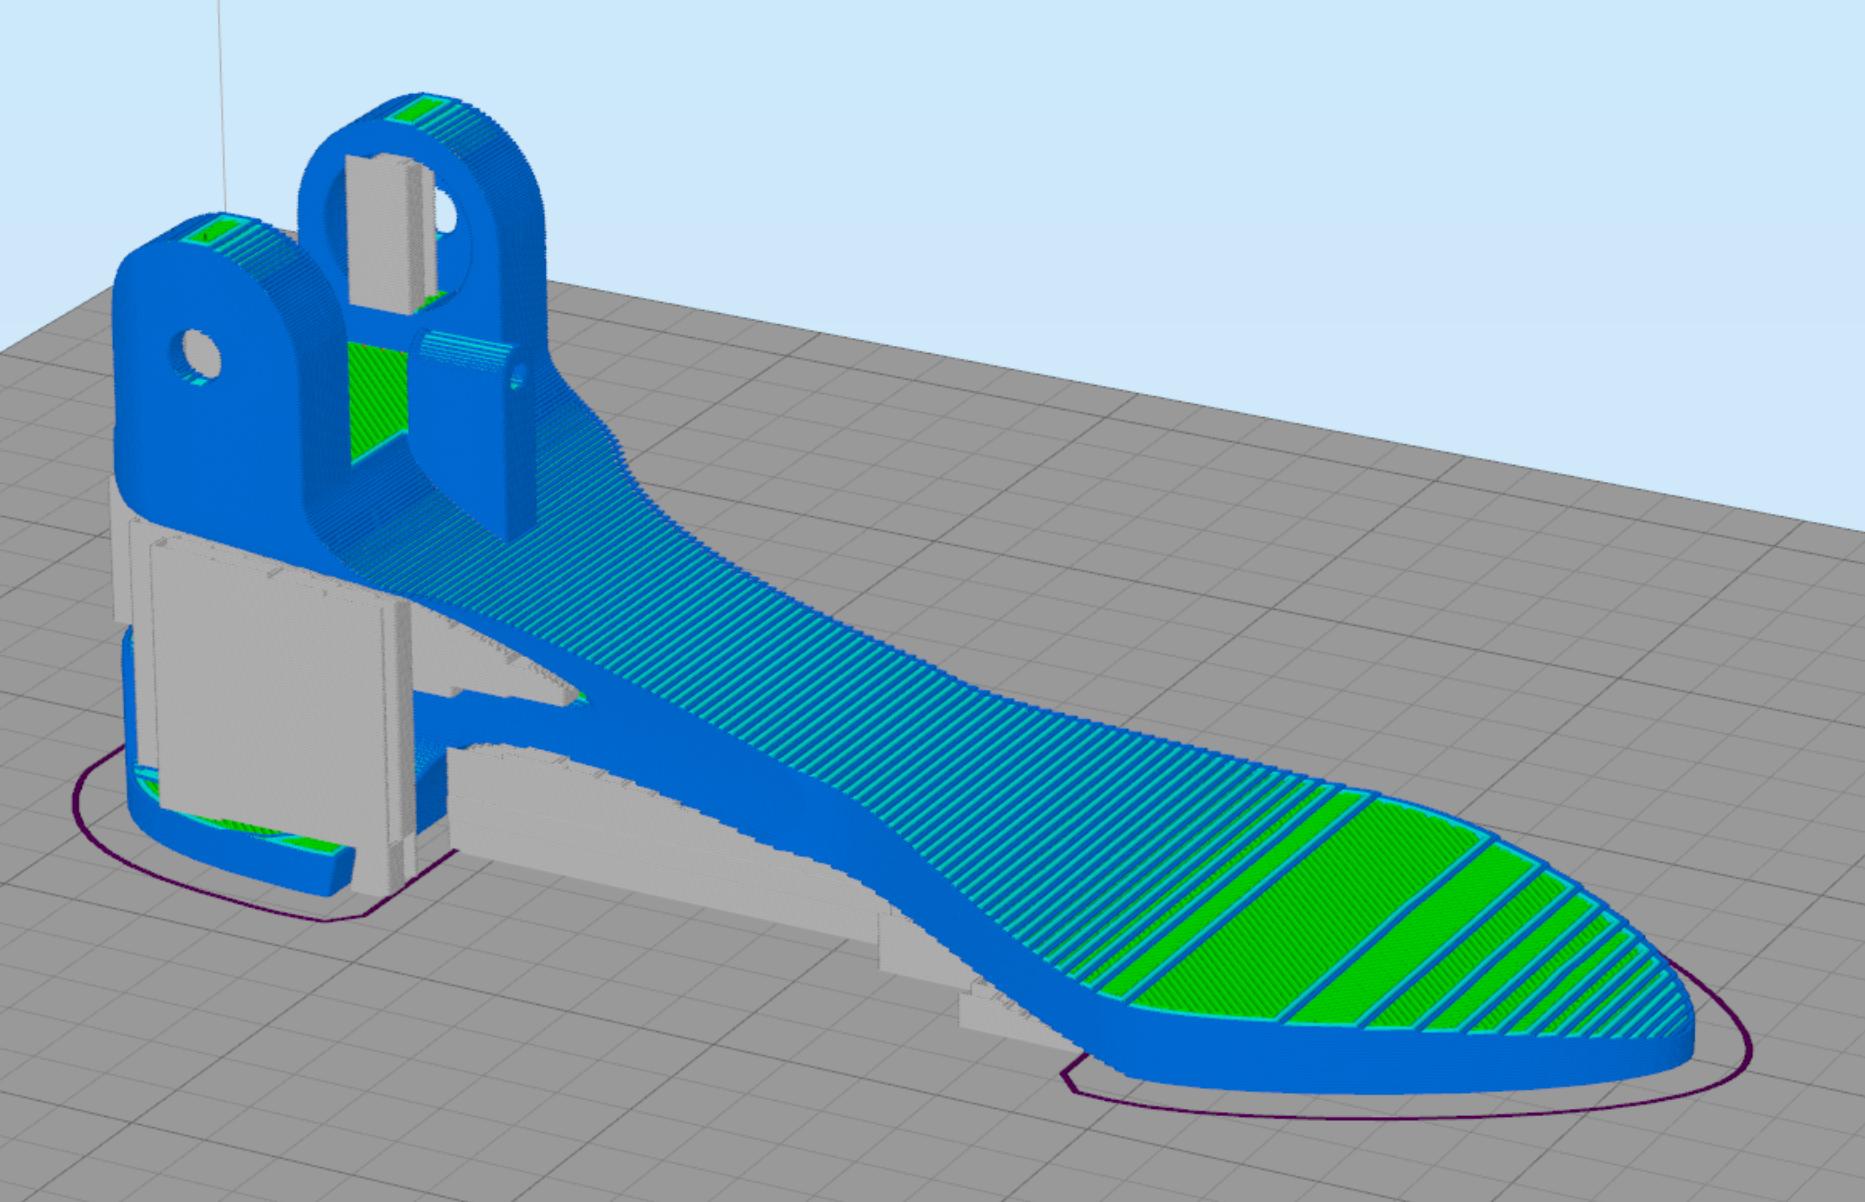
\includegraphics[width=0.75\textwidth]{figures/3d_printing_gcode}
  \caption{Gcode visualization from Simplify3D \cite{simplify3d}.}
  \label{fig:3d_printing_gcode}
\end{figure}
One of the intrinsic problems of this technology is the need of material support for some of the meshes.
Due to its stratification technique, if one of the higher layers lacked a lower one to be supported on, the material would fall causing problems in final part.
Nowadays, mostly all the slicers offer a material support solution that can vary but generally offering good results.
The Figure \ref{fig:photo_material_support} depicts two feet, one with material support and the other with it removed.

All the parts have been individually adjusted until the clearances have been as expected.
This has been achieved by an recursive process and a mix between experimental tests and other tools like the presented in \ref{sub:arc_compensation}.
In the Figure \ref{fig:photo_3d_printed} a detail of actual parts 3D printed and assembled in the robot are shown.

\begin{figure}[ht]
    \centering
    \begin{subfigure}[b]{0.49\textwidth}
        \includegraphics[width=\textwidth]{figures/photo_material_support.jpg}
        \caption{Feet with and without material support.}
        \label{fig:photo_material_support}
    \end{subfigure}
    \begin{subfigure}[b]{0.49\textwidth}
        \includegraphics[width=\textwidth]{figures/photo_3d_printed.jpg}
        \caption{Detail of 3D printed parts assembled.}
        \label{fig:photo_3d_printed}
    \end{subfigure}
    \caption{Photos of 3D printed parts.}
\end{figure}

  \subsection{Arc compensation in FFF} % (fold)
  \label{sub:arc_compensation}
  For the CAD models of the 3D printed parts, the clearances of the internal holes have been adjusted following \cite{arc_compensation}.
  The undersizing of internal holes is a common problem in this sort of technology due to the lack of information of the common-used exporting format: the STL.
  This only contains the 3D model expressed as a set of external triangles and its normal, which difficulties the correction of malformations inherent to this technology.

  In the case of the Fused Filament Fabrication (FFF), the material is extruded equally in both sides of the arc, as shown in \ref{fig:arc_compensation}. 
  However, in the side of the smaller curve, less material is needed.
  This correction can be calculated with the equation \ref{eq:r_arc_compensation}   being $t$ the noozle diameter, $R$ the desired internal hole radius and $r$ the corrected radius.
  \begin{equation}
    \label{eq:r_arc_compensation}
    r=\frac{t+\sqrt{t^2+4R^2}}{2}
  \end{equation}
  As an example, Klee suggests an internal hole of 4.4 mm in the case of the selected nuts \cite{klee}. 
  Thus, the diameter in the CAD model has been adjusted for this data and a noozle of 0.4 mm. The result is then show in \ref{eq:diameter_example}.

  \begin{equation}
    \label{eq:diameter_example}
    d=2r=\frac{t+\sqrt{t^2+4R^2}}{2}=0.4+\sqrt{0.4^2+4*2.2^2}=4.81
  \end{equation}

  \begin{figure}[tb]
    \centering
    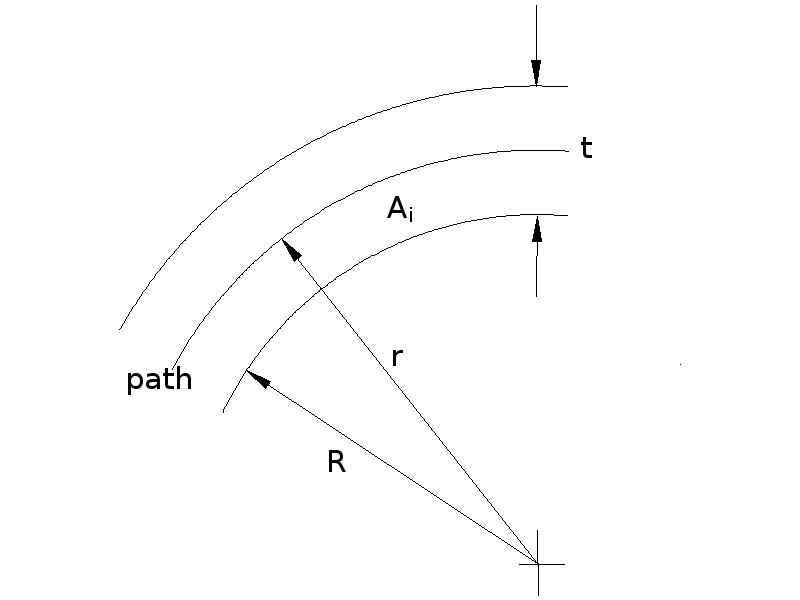
\includegraphics[width=0.5\textwidth]{figures/Arc-compensation}
    \caption{Technical representation of the generated arc when using FFF technology.}
    \label{fig:arc_compensation}
  \end{figure}
  % subsection arc_compensation (end)

% section 3d_printing (end)

%!TEX root = ../../../report.tex
\section{Machining} % (fold)
\label{sec:machining}
This section presents the process of machining followed for the non 3D-printed components that required some extra treatment during the assembly of the robot.
The need of use of these parts is justified by the fact that the 3D printers used have a limited printing volume.
Additionally, the mechanical properties given by the PLA did not satisfy all the requirements of all the parts.
The rods of the joint axes, the beams used to create the holding structure or the carbon fiber tubes are some examples of these requirements of size and mechanical constraints.

The original carbon fiber tubes have been manually cut and drilled to give them their final configuration.
Special attention has been paid to the symmetry of the frame during the construction following the design criteria established in \ref{sec:physical_properties}.
The joints axes rods have been also manually cut and filed according to the design.
Besides, the holding structure mounted over the treadmill has been cut and assembled by hand as well.
Knowing that this kind of operations is human error prone, the number of parts on the frame that needed to be manually produced has been tried to be minimized during the design.
The drawings for such parts are included as appendices in \ref{app:mechanical_drawings}.

% section machining (end)
%!TEX root = ../../../report.tex
\section{PCBs and wiring} % (fold)
\label{sec:pcbs_and_wiring}
In order to reduce weight and inertias, \ref{ssub:extension_pcbs} presented an extension board that interfaces between the motor and the BLDC electronics.
With a 1.8 meter long wiring used to extend the connection, the purpose of the extension PCBs are to be mounted over the joints, close enough to the motors so that their original wiring can be used, as in Figure \ref{fig:pcb2}, and transfer the signals to the motor board out of the structure, as in Figure \ref{fig:electronics1}.

New Molex connectors have been soldered to the original boards in order to implement these extensions, as shown in Figure \ref{fig:electronics2} within the final arrangement of the motor boards and the main processor board.
A distinctive color has been chosen for the wiring of each motor just to ease the task of arranging the final configuration.
Every motor board is labeled with the name of the joint it drives and matched to the appropriate address from the main processor by software, as explained in \ref{sub:ros_control_hardware_locokit_interface}.
This means that if a BLDC motor board is going to be changed, both its physical connection, label and internal address have to be changed accordingly.

All the off-board electronics has been placed over a small wooden structure to ease its use.

\begin{figure}[ht]
\centering
  \begin{subfigure}[b]{0.4\textwidth}
    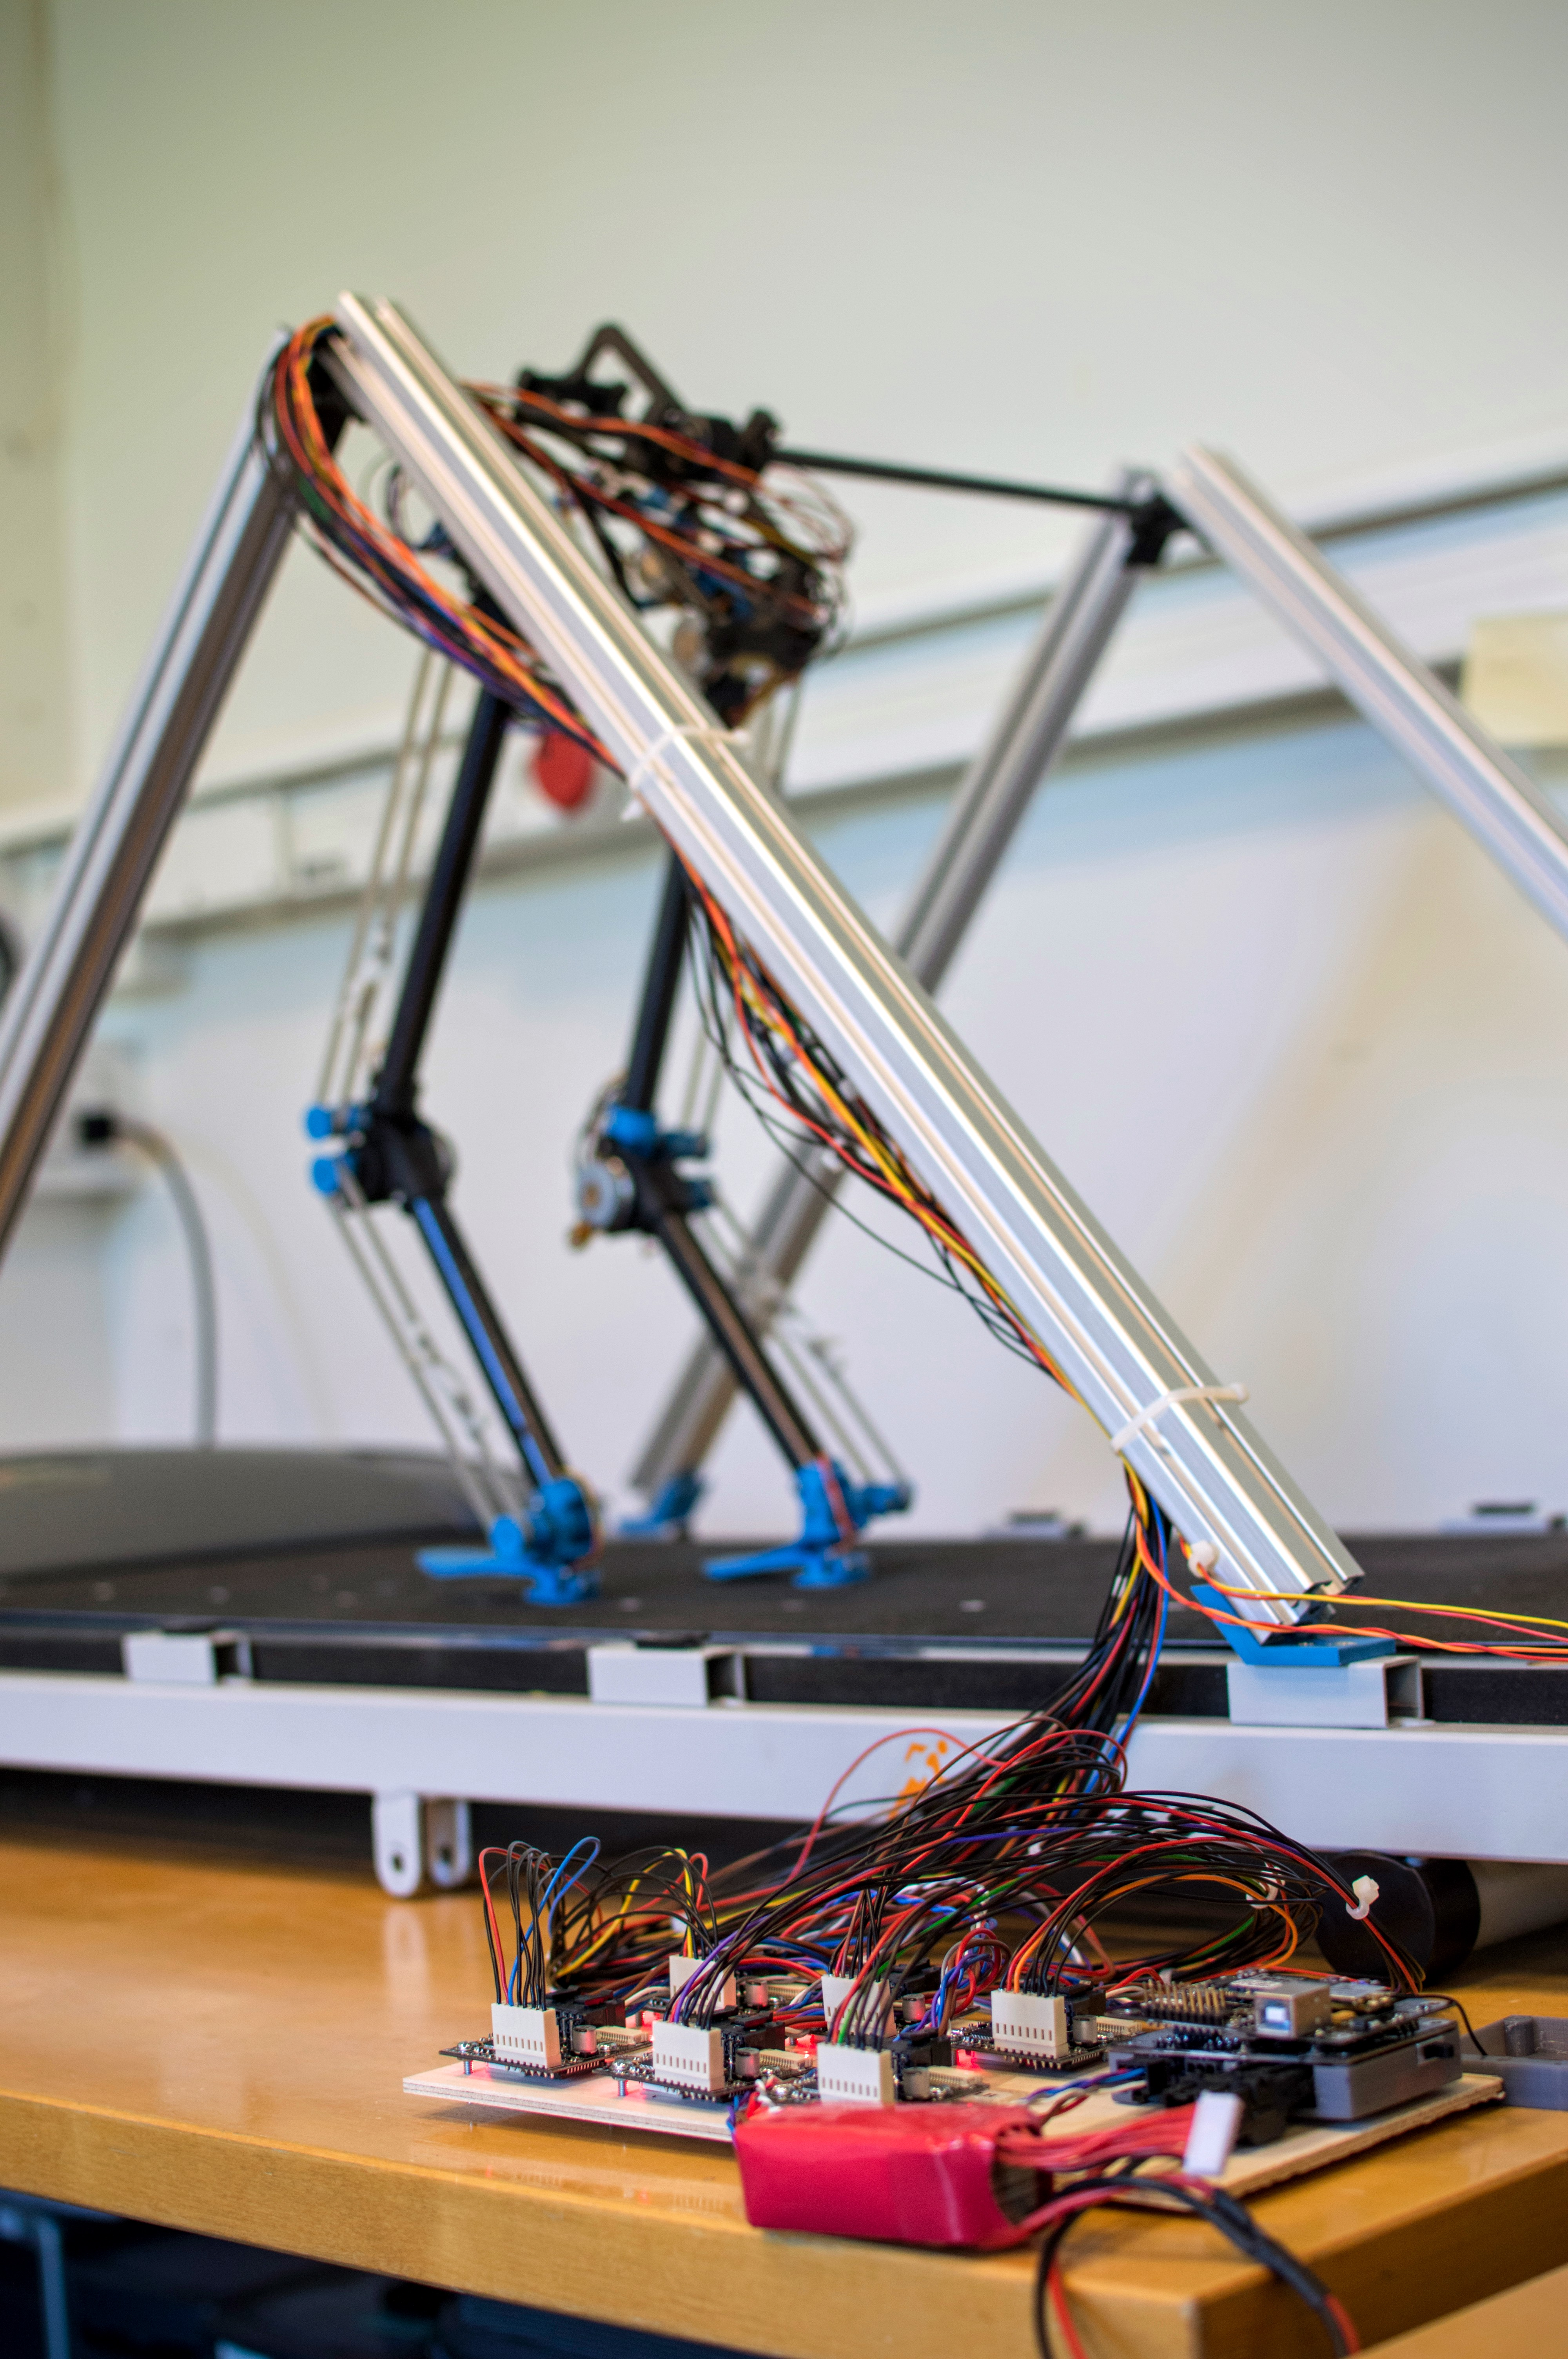
\includegraphics[width=\textwidth]{figures/photo_electronics_2.jpg}
    \caption{Wiring on the structure}
    \label{fig:electronics1}
  \end{subfigure}
  \begin{subfigure}[b]{0.4\textwidth}
    \includegraphics[width=\textwidth]{figures/photo_electronics.jpg}
    \caption{Electronics main board}
    \label{fig:electronics2}
  \end{subfigure}
  \begin{subfigure}[b]{0.4\textwidth}
    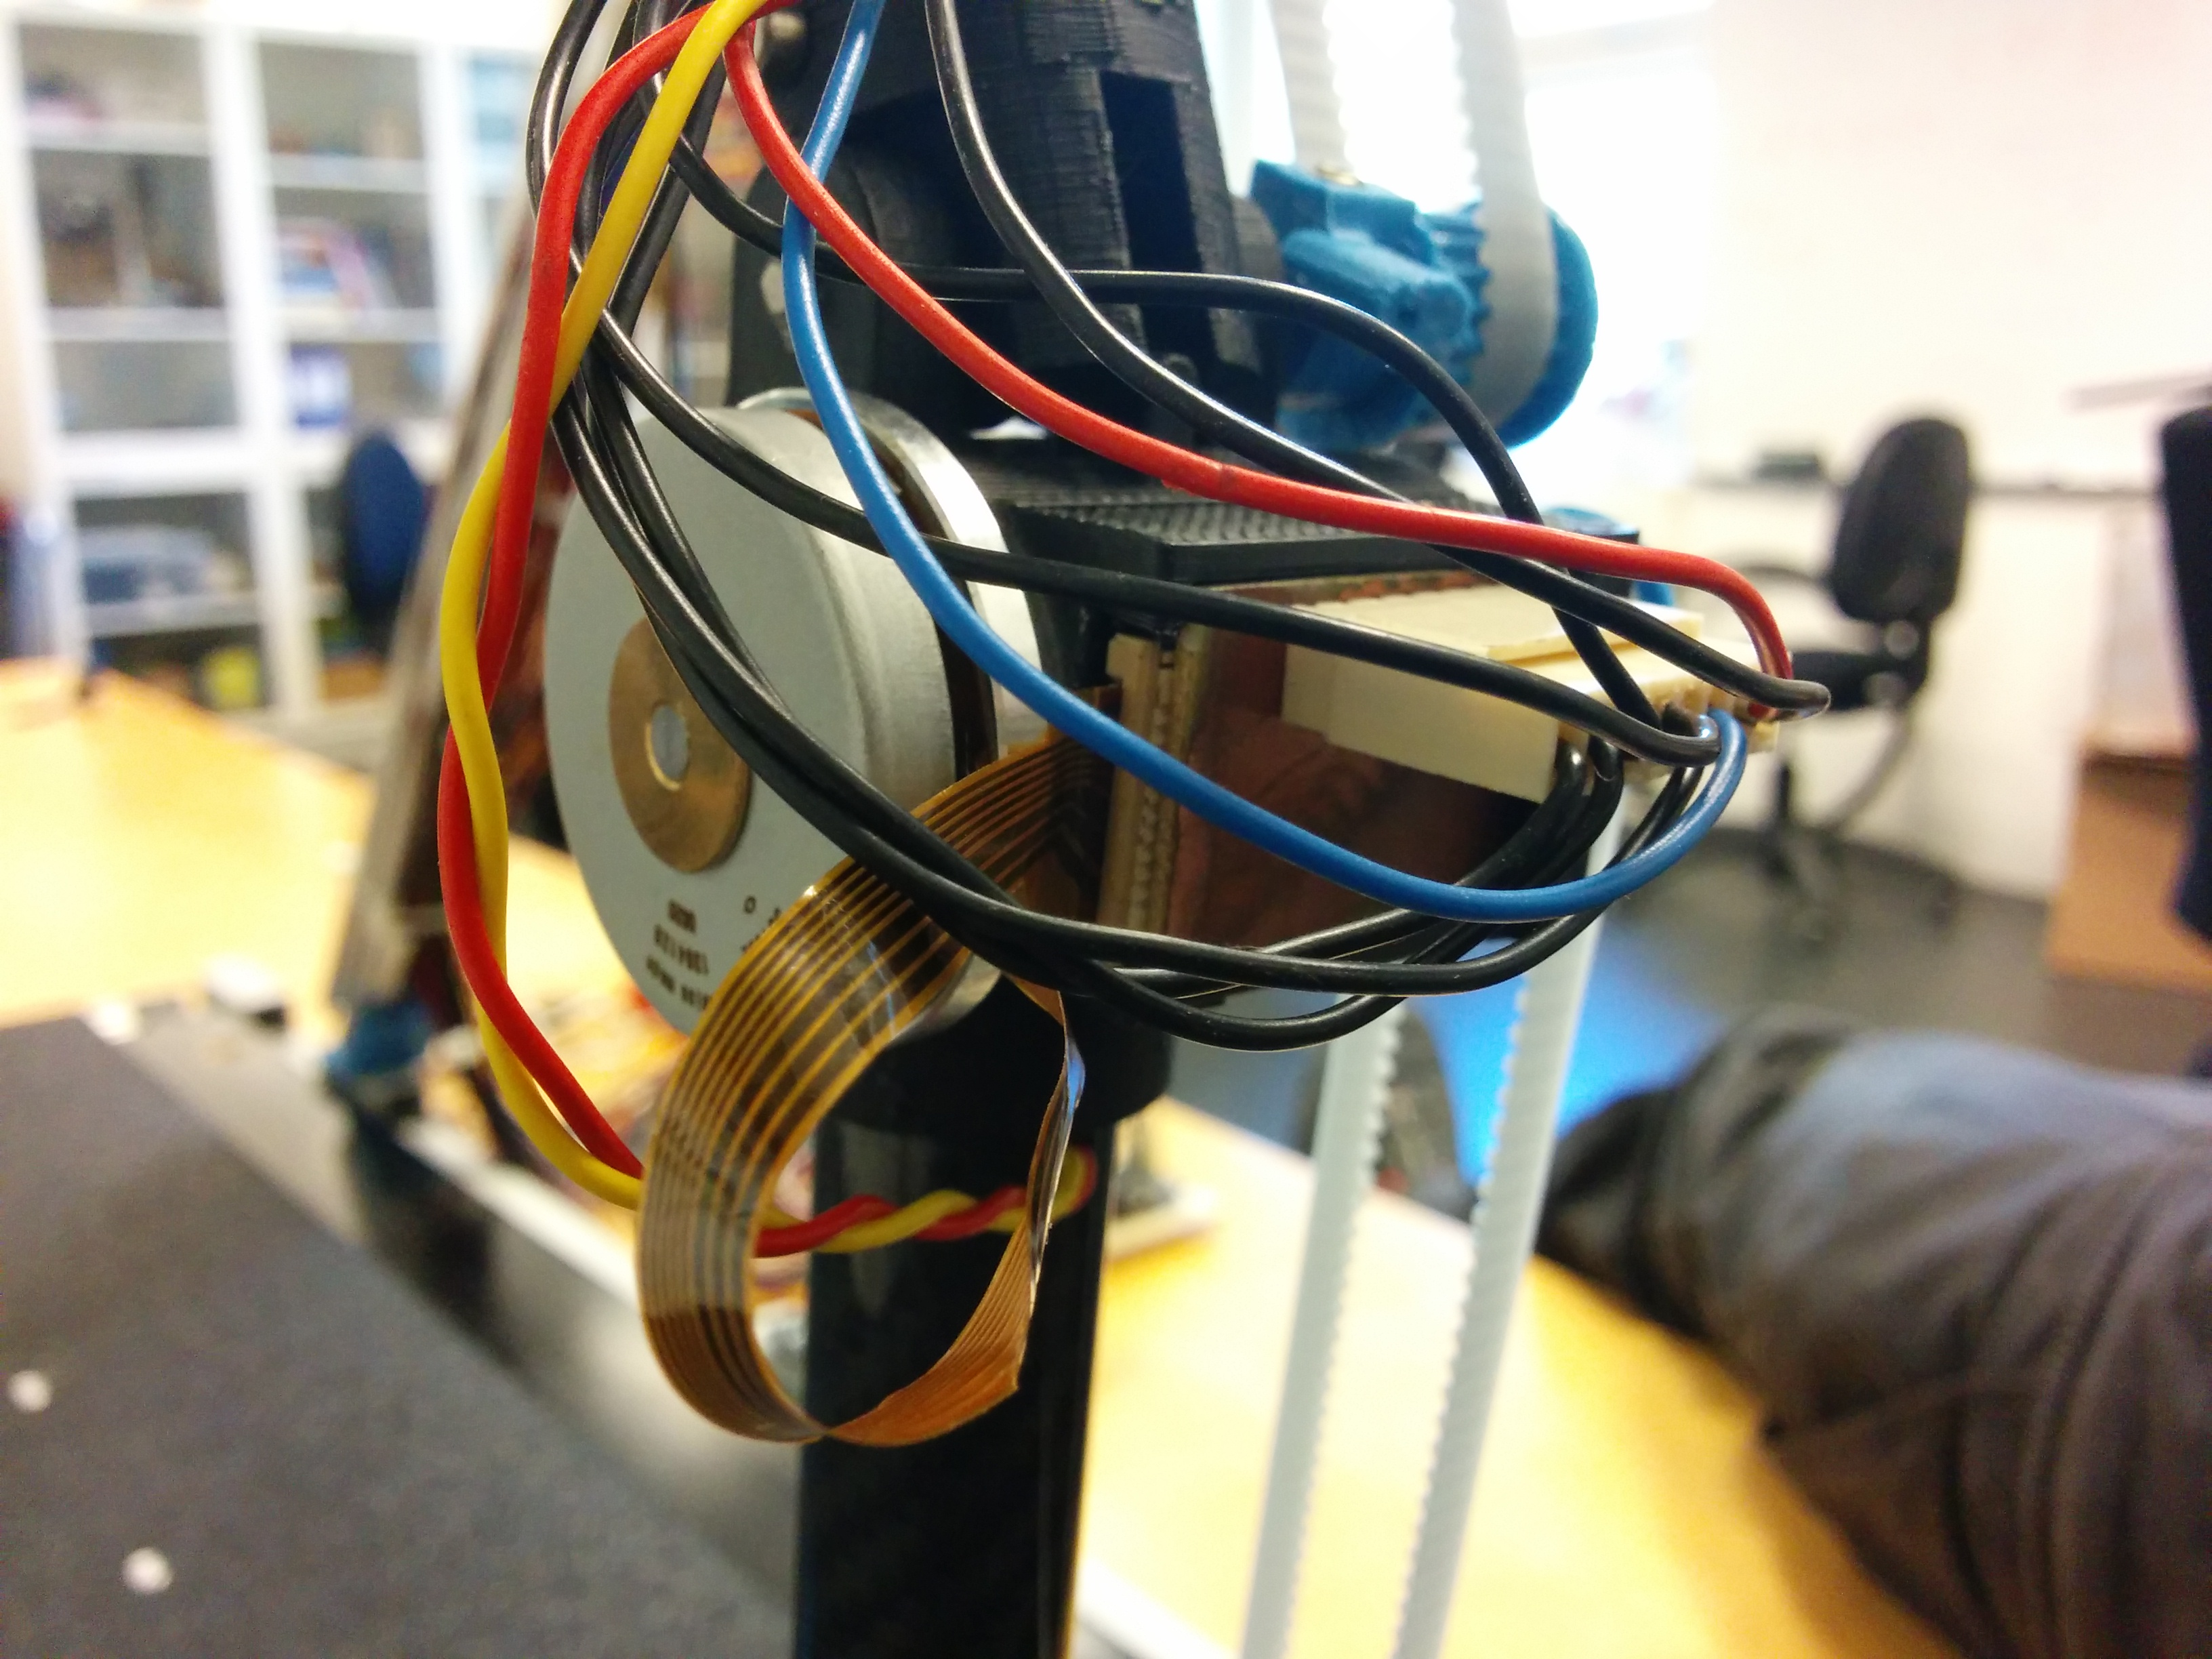
\includegraphics[width=\textwidth]{figures/photo_electronics_detail.jpg}
    \caption{Left leg extension PCB implemented}
    \label{fig:pcb2}
  \end{subfigure}
  \caption{Final architecture of electronics}
\end{figure}

% section pcbs_and_wiring (end)
%!TEX root = ../../../report.tex
\section{Providers} % (fold)
\label{sec:providers}
As explained in the management of the project section \ref{sec:project_management}, all the components that could not be manufactured or were not available at the university facilities had to be ordered.
The providers have been selected among the range offered by the Mærsk Mc-Kinney Møller Institute.
The main selection criteria of utilized external components has been standardization.
Following the underlying principles of this project, only low-cost, standard pieces have been acquired. As an example, RuBi only needs three types of screws (only M3 metric) and one kind of bearing.
A list with all the components bought and its providers is shown in the Table \ref{tab:material_cost}. 

\subsection{Components delivery} % (fold)
\label{sub:components_delivery}
In the initial scheduling of the project, conducted at its very beginning, it was planned to have defined and ordered by the end of April all the necessary components that had to be bought.
This was decided assuming that the delivery of the parts could take up to three weeks in a reasonable scenario.
The acquisition of external components was considered during the planning of the project as a strong time constraint, and the rest of the workflow was scheduled to adapt to this step.
However, despite the fact that most of the parts were received within the first few week after ordering, the springs suffered a severe delay that prevented their scheduled assembly and produced a necessary reschedule of the project flow in order to adapt to this.
This event has mainly impeded carrying out the devised experiments presented in \ref{cha:experiments} and some basic performance tests that were considered essential.
This is further discussed in \ref{cha:results} and \ref{cha:discussion}.

% subsection components_delivery (end)

% section providers (end)
%!TEX root = ../../../report.tex
\section{Assembly} % (fold)
\label{sec:assembly}
Due to the fact that basically all the parts have been linked making use of 3D-printed parts, and all the tolerances of these have been adjusted individually, the assembly has been found easy and fast.
The mounting process has proved to be rapid enough to change some of the parts, as the springs, within minutes.
Furthermore, in the event of mechanical failure of any of the 3D-printed parts, its production and replacement is simple enough to reduce the maintenance time.
This result of employing 3D-printed parts can be considered as one of the main advantages of the whole platform.
The tension of the belts have been adjusted experimentally as explained in the section \ref{sub:pulleys_and_belts} using the zip ties installed.
In Figure \ref{fig:photo_robot_walking}, the complete robot assembled is shown while in \ref{fig:photo_dacbot}, a size comparison between the DACbot \cite{dacbot1} and RuBi can be done.

\begin{figure}[ht!]
    \centering
    \begin{subfigure}[b]{0.49\textwidth}
        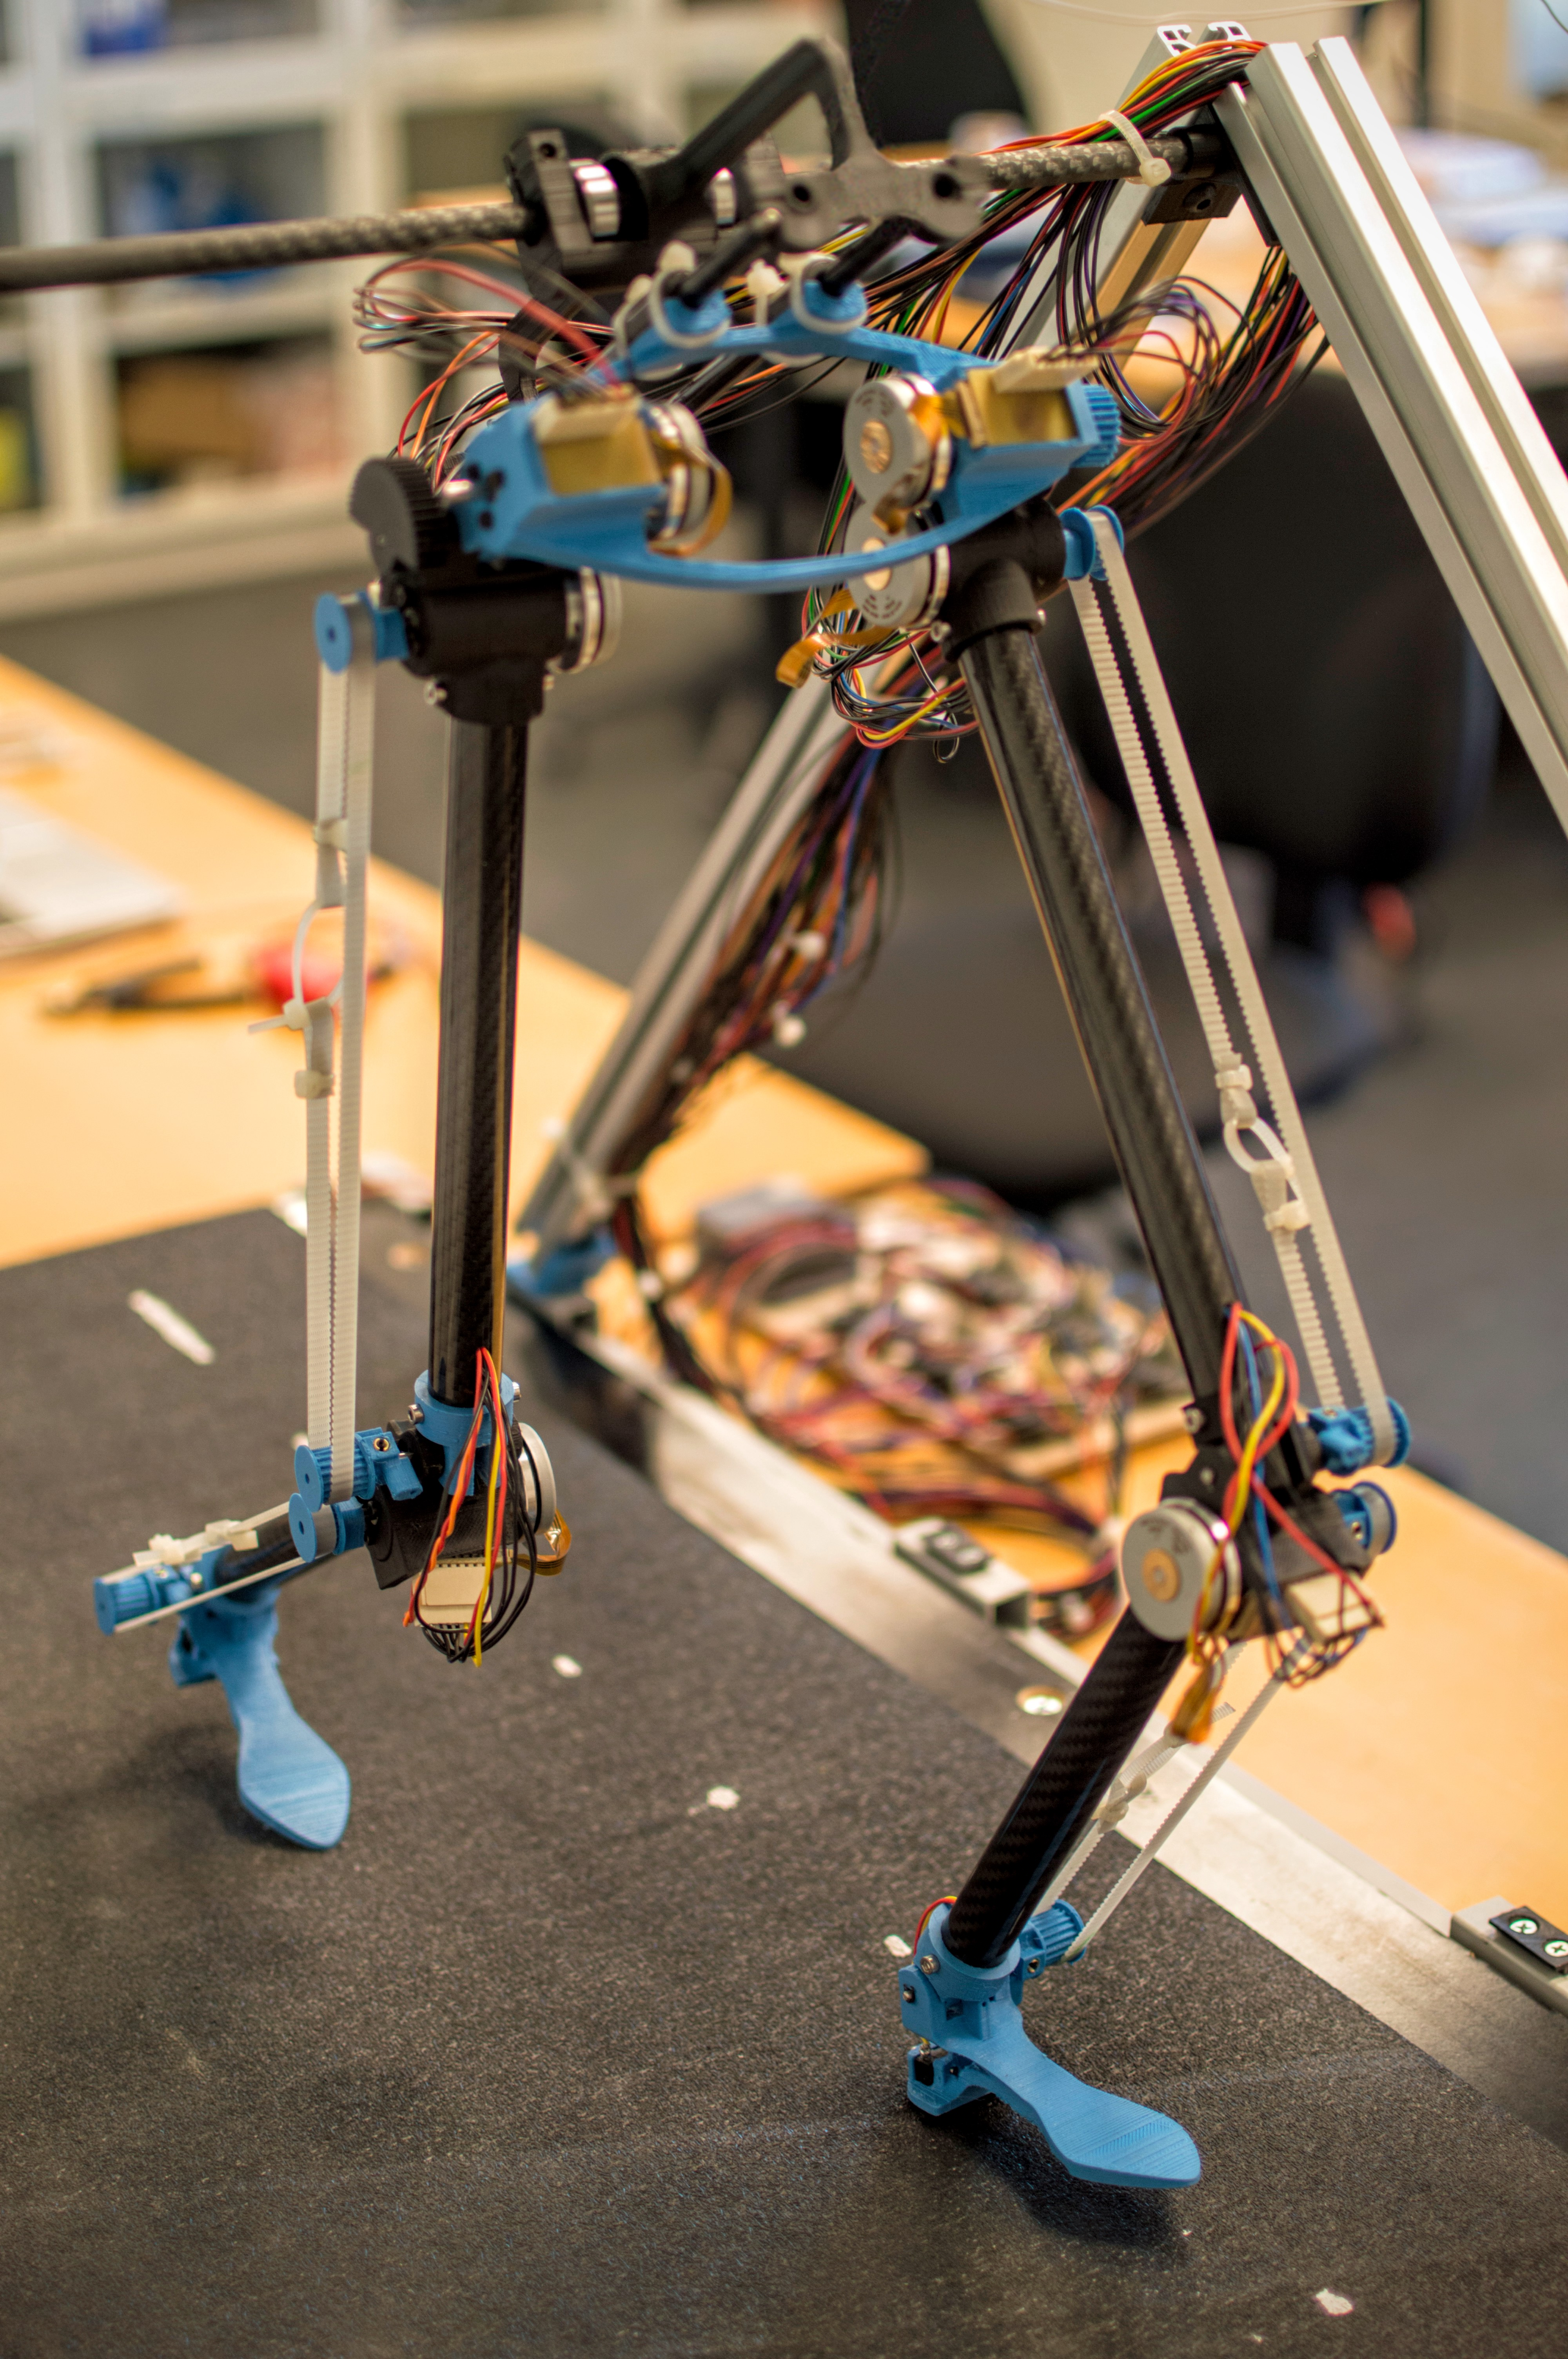
\includegraphics[width=\textwidth]{figures/photo_robot_walking.jpg}
        \caption{RuBi assembled}
        \label{fig:photo_robot_walking}
    \end{subfigure}
    \begin{subfigure}[b]{0.49\textwidth}
        \includegraphics[width=\textwidth]{figures/photo_dacbot.jpg}
        \caption{RuBi and DACbot over the same treadmill}
        \label{fig:photo_dacbot}
    \end{subfigure}
\end{figure}    
% section assembly (end)
%%!TEX root = ../../../report.tex
\section{How to bring up the robot} % (fold)
\label{sec:how_to_bring_up_the_robot}
In order to bring up the robot, a battery has to power it and the computer must be started.
It will automatically create a Wi-Fi hotspot called \textit{RuBi} where the user can connect to.
From this moment, the robot should be able to receive motor commands.
If not, the IP in the \textit{locokit\_hw} has to be changed according to the stablished in the host.
In the guest, open a new terminal and run:

\begin{lstlisting}
roslaunch rubi_bringup rubi_bringup.launch
\end{lstlisting}

ROS Control will be loaded along with the locokit hardware interface and the controllers can move the real robot.
% section how_to_bring_up_the_robot (end)

% chapter implementation (end)